\documentclass[tikz,border=10pt]{standalone}
\usepackage[T1]{fontenc}
\usepackage{mathpazo}
\usepackage{amsmath,amssymb}
\usetikzlibrary{arrows.meta, positioning, calc, fit, shapes.geometric}

\definecolor{stblue}{HTML}{7B97AD}
\definecolor{rwgold}{HTML}{B8995E}
\definecolor{sage}{HTML}{7A9A7E}
\definecolor{dkbrown}{HTML}{3D3530}
\definecolor{wmgray}{HTML}{7B7067}
\definecolor{cream}{HTML}{F9F6F0}
\definecolor{border}{HTML}{D4C9B8}
\definecolor{terracotta}{HTML}{C47A6A}

\begin{document}
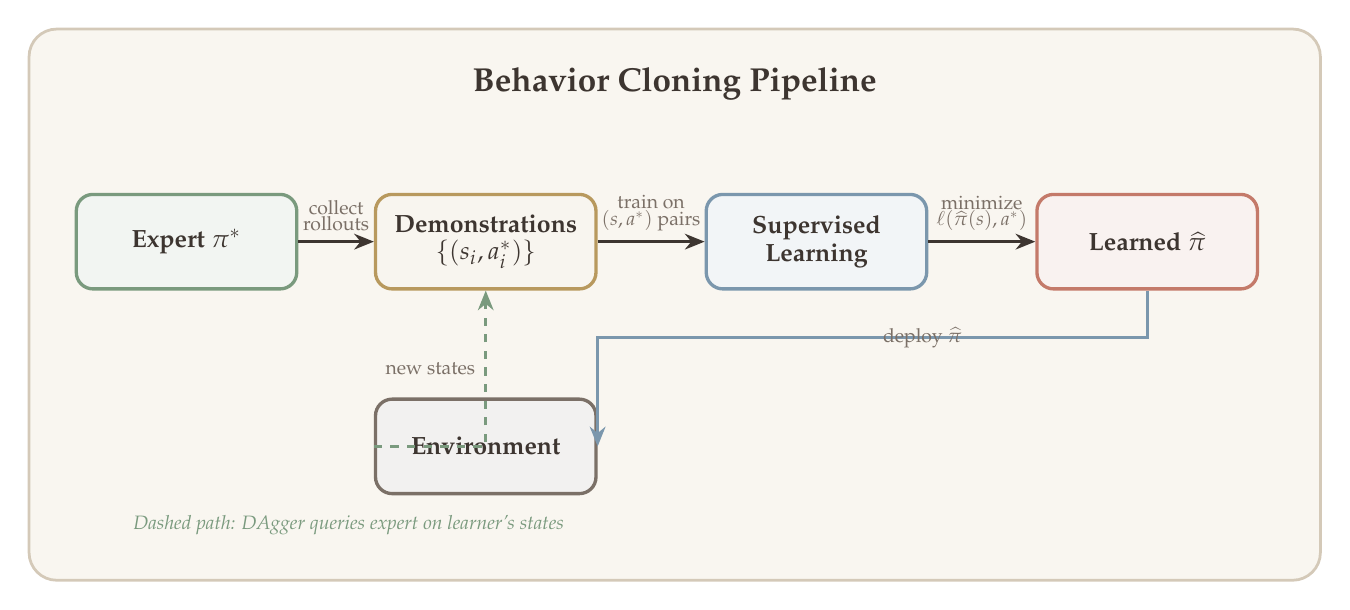
\begin{tikzpicture}[
  >={Stealth[length=2.5mm, width=2mm]},
  box/.style={draw=#1, line width=1.2pt, fill=#1!10, rounded corners=6pt,
    minimum width=28mm, minimum height=12mm, font=\small\bfseries,
    text=dkbrown, align=center, inner sep=4pt},
  arr/.style={->, line width=1pt, dkbrown},
  lbl/.style={font=\scriptsize, text=wmgray, align=center},
]

% Background
\fill[cream, rounded corners=10pt] (-1.2,-3.5) rectangle (15.2,3.5);
\draw[border, rounded corners=10pt, line width=1pt] (-1.2,-3.5) rectangle (15.2,3.5);

% Title
\node[font=\large\bfseries, text=dkbrown] at (7.0,2.8) {Behavior Cloning Pipeline};

% === Top row: Expert -> Demonstrations -> Supervised Learning -> Learned Policy ===

\node[box=sage] (expert) at (0.8,0.8) {Expert $\pi^*$};
\node[box=rwgold] (demos) at (4.6,0.8) {Demonstrations\\[-1pt]$\{(s_i, a_i^*)\}$};
\node[box=stblue] (sl) at (8.8,0.8) {Supervised\\[-1pt]Learning};
\node[box=terracotta] (policy) at (13.0,0.8) {Learned $\widehat{\pi}$};

\draw[arr] (expert) -- (demos) node[midway, above, lbl] {collect\\[-2pt]rollouts};
\draw[arr] (demos) -- (sl) node[midway, above, lbl] {train on\\[-2pt]$(s,a^*)$ pairs};
\draw[arr] (sl) -- (policy) node[midway, above, lbl] {minimize\\[-2pt]$\ell(\widehat\pi(s), a^*)$};

% === Bottom row: Environment interaction (for DAgger) ===

\node[box=wmgray] (env) at (4.6,-1.8) {Environment};

\draw[arr, stblue] (policy.south) -- ++(0,-0.6) -| (env.east)
  node[pos=0.25, right, lbl] {deploy $\widehat\pi$};
\draw[arr, sage, dashed] (env.west) -| (demos.south)
  node[pos=0.75, left, lbl] {new states};

% DAgger label
\node[font=\scriptsize\itshape, text=sage, anchor=west] at (0.0,-2.8)
  {Dashed path: DAgger queries expert on learner's states};

\end{tikzpicture}
\end{document}
